\documentclass[a4paper,11pt]{jsarticle}
\usepackage[a4paper]{geometry}
\usepackage{multirow}
\usepackage{ascmac}
\usepackage[dvipdfmx]{graphicx}
\geometry{left=15mm, right=15mm, top=15mm, bottom=15mm}

\newcommand{\hwVer}{Ver 1.0}
\newcommand{\fwVer}{Ver 1.0}
\newcommand{\midTrue}{○}
\newcommand{\midFalse}{×}

\begin{document}
\begin{titlepage}
\title{\vspace*{60mm}\ \\HTLAB.NET Arduino DRSSTC Interrupter \hwVer \\(Firmware \fwVer)}
\author{\vspace*{80mm}\ \\つくば科学株式会社\\菊地 秀人}
\date{\vspace*{20mm}\ \\2019年12月11日}
\maketitle
\thispagestyle{empty}
\end{titlepage}
\clearpage



\section{各部の名称と機能}

\vspace*{10mm}
\begin{center}

\includegraphics[width=100mm]{image/Arduino_Interrupter_v1_Design.png}
\end{center}
\vspace*{10mm}

\begin{table}[htbp]
\begin{center}
\begin{tabular}{ | c | c | c | c | }
\hline
\textbf{名称} & \textbf{種別} & \textbf{概要} \\\hline
OUT1 / 2 & BNC出力端子およびLED & テスラコイルへの接続に使用。信号出力時にLEDが点灯。 \\\hline
POWER & トグルスイッチ & インタラプター本体の電源操作に使用。 \\\hline
MIDI(SW1) & トグルスイッチ & インタラプターモードとMIDIモードの切替に使用。 \\\hline
MODE(SW2) & トグルスイッチ & それぞれの拡張モードの切替に使用。 \\\hline
PUSH1 / 2 & プッシュスイッチ & 主にワンショットモードの出力時に使用。 \\\hline
VR1 - 4 & ボリューム & 値の設定に使用。 \\\hline
USB & USB端子 & コンピューターとの接続に使用。USB-MIDI使用可能。 \\\hline
MIDI IN & MIDI端子 & MIDI機器との接続に使用。チャンネル設定可能。 \\\hline
MIDI OUT & MIDI端子 & MIDI機器との接続に使用。MIDI-THRU動作。 \\\hline
\end{tabular}
\end{center}
\end{table}


\clearpage


\section{電源の操作}

\subsection{電源の入れ方}

POWERスイッチをONにします。

\vspace*{10mm}
\begin{center}

\includegraphics[width=100mm]{image/Arduino_Interrupter_v1_LCD.png}
\end{center}
\vspace*{10mm}

スプラッシュスクリーンが表示され、インタラプターが起動します。 \\
起動しない場合は、内蔵電池(単3電池 * 6本)を確認してください。 \\

\vspace*{5mm}


\subsection{電源の切り方}

POWERスイッチをOFFにします。 \\

\vspace*{5mm}


\subsection{USB電源を使う}

USBケーブルにてコンピューター等に接続することによってUSB電源を使用することができます。 \\
この際、POWERスイッチの状態に関わらずUSB接続が優先されます。 \\
POWERスイッチがOFFの状態でも、USBを接続することによって電源がONになります。 \\
POWERスイッチがONの場合にUSB接続を行うと、内蔵電池との接続が切り離されUSB電源供給に切り替わります。 \\

\vspace*{5mm}

\begin{itembox}[l]{\textbf{注意事項}}
POWERスイッチがONでUSB接続中の場合、USBケーブルを抜いた際にリセットがかかります。 \\
テスラコイルの操作中は注意してください。
\end{itembox}

\vspace*{5mm}

\begin{itembox}[l]{\textbf{注意事項}}
POWERスイッチがONでUSB接続中の場合、内蔵電池との接続は自動的に切り離されますが、数mA程度の微小電流が内蔵電池から消費されます。 \\
長期間使用する場合はPOWERスイッチをOFFにすることを推奨します。
\end{itembox}



\clearpage


\section{モード切替の方法}

MIDIスイッチ(SW1)・MODEスイッチ(SW2)を操作することによって動作モードを変更します。 \\
設定によってはインタラプターモード時にVR4を操作することにより拡張モードを使用可能です。 \\


\vspace*{5mm}
\begin{center}

\includegraphics[width=100mm]{image/Arduino_Interrupter_v1_Design_Interface.png}
\end{center}
\vspace*{5mm}


\begin{table}[htbp]
\begin{center}
\begin{tabular}{ | c | c |  c | }
\hline
\textbf{MIDIスイッチ(SW1)} & \textbf{MODEスイッチ(SW2)} & \textbf{操作モード} \\\hline
OFF & OFF & インタラプターモード \\\hline
OFF & ON & バーストモード \\\hline
ON & OFF & MIDI モード \\\hline
ON & ON & MIDI FIXED モード \\\hline
\end{tabular}
\end{center}
\end{table}


後述する設定を利用することにより、インタラプターモード時に拡張モードを使用することが出来ます。 \\


\begin{table}[htbp]
\begin{center}
\begin{tabular}{ | c | c | c | c | }
\hline
\textbf{VR4回転位置} & \textbf{4-MODE設定時} & \textbf{2-MODE設定時} & \textbf{1-MODE設定時}  \\\hline
0-25\% & インタラプターモード & インタラプターモード & インタラプターモード \\\hline
25-50\% & ワンショットモード & インタラプターモード & インタラプターモード \\\hline
50-75\% & ハイパワーモード & ワンショットモード & インタラプターモード \\\hline
75-100\% & ハイパワーワンショットモード & ワンショットモード & インタラプターモード \\\hline
\end{tabular}
\end{center}
\end{table}


\begin{itembox}[l]{\textbf{注意事項(テスラコイル焼損の恐れあり)}}
「4-MODE」設定時:バーストモードからインタラプターモードにモード切替を行う際に、VR4の位置が50-75\%の位置にある場合ハイパワーモードに切り替わります。 \\
テスラコイルの焼損を防ぐために、バーストモード使用後は必ずVR4の回転位置を0\%に戻してから、インタラプターモードに切り替えてください。 \\
\textbf{\underline{ハイパワーモードを使用しない場合は、「2-MODE」または「1-MODE」設定を使用することを推奨します。}}
\end{itembox}



\clearpage

\section{インタラプターモード}

設定した周波数・ON時間の信号を出力する標準的なモードです。

\subsection{画面表示}

画面2行目に出力周波数とON時間が表示されます。 OUT1 / 2 同時に同じ信号が出力されます。

\vspace*{5mm}
\begin{center}
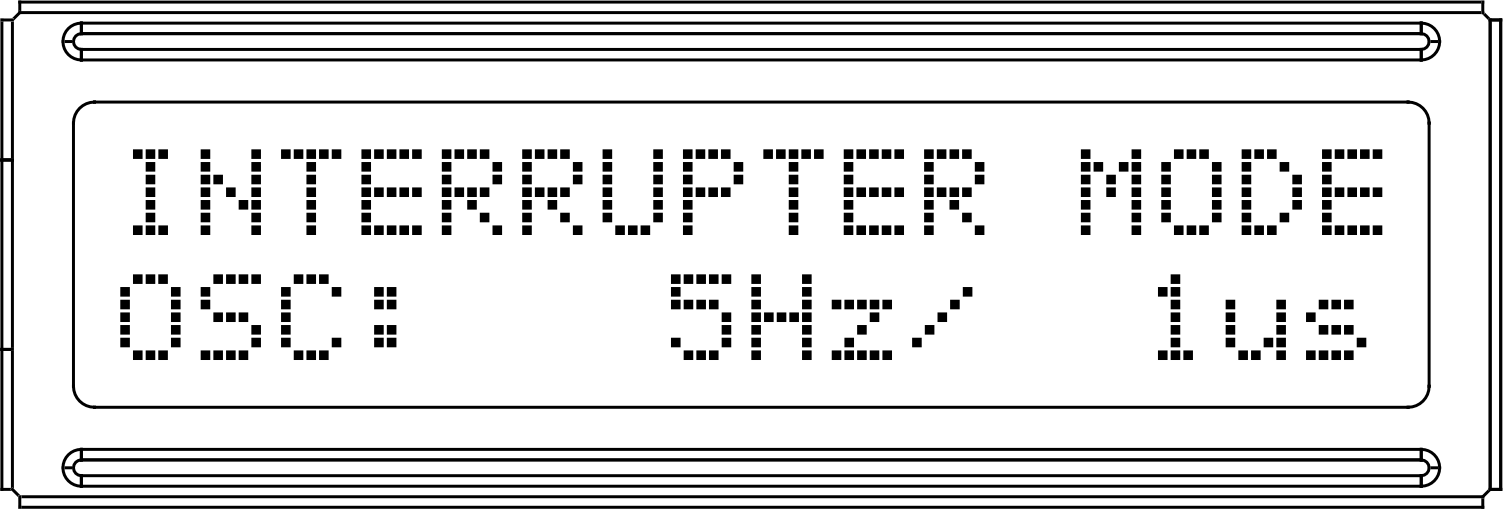
\includegraphics[width=100mm]{image/Arduino_Interrupter_v1_LCD_INT.png}
\end{center}
\vspace*{5mm}

\subsection{操作方法}

\vspace*{5mm}
\begin{center}

\includegraphics[width=100mm]{image/Arduino_Interrupter_v1_Design_Interrupter.png}
\end{center}
\vspace*{5mm}

基本的にVR1とVR2を操作することにより周波数とON時間を設定します。

\vspace*{5mm}

\begin{table}[htbp]
\begin{center}
\begin{tabular}{ | c | c | }
\hline
\textbf{VR1} & 周波数変更(5Hz - 1018Hz @ 1Hz Step) \\\hline
\textbf{VR2} & ON時間変更(1us - 254us @ 1us Step) \\\hline
\textbf{VR3} & 割当無し \\\hline
\textbf{VR4} & モード切替(4-MODE / 2-MODE時) \\\hline
\textbf{PUSH1} & 割当無し \\\hline
\textbf{PUSH2} & 割当無し \\\hline
\end{tabular}
\end{center}
\end{table}



\clearpage

\section{ワンショットモード}

プッシュボタンの操作で任意タイミングの信号を出力するモードです。

\subsection{画面表示}

画面2行目に OUT1 / 2 それぞれのON時間が表示されます。

\vspace*{5mm}
\begin{center}
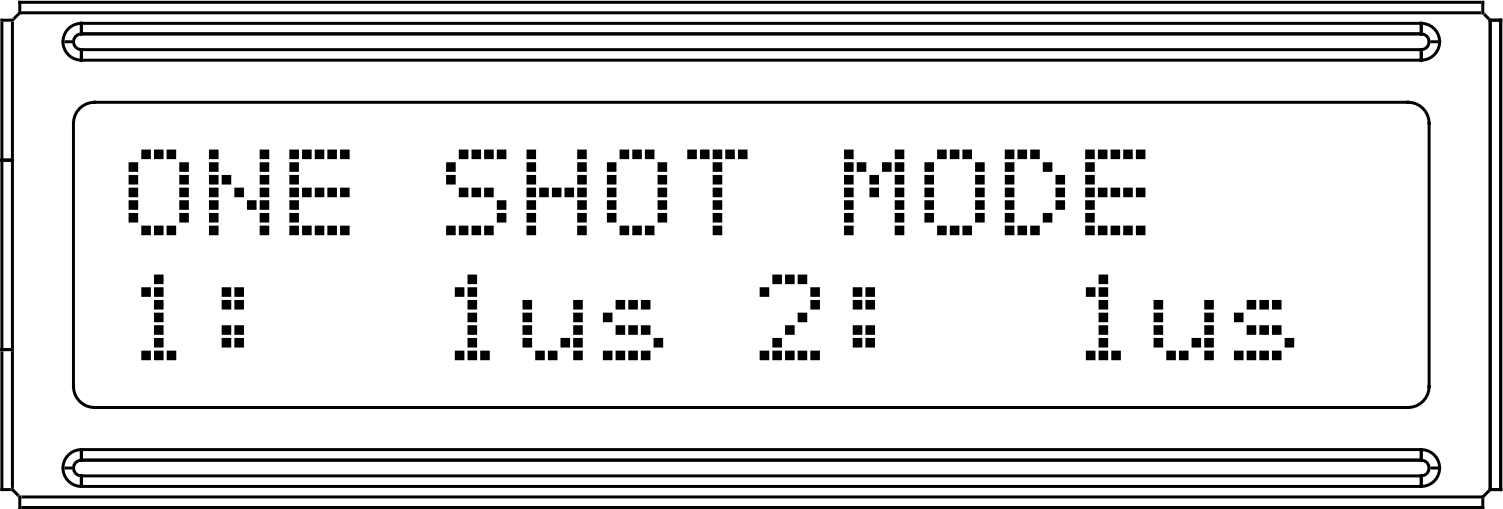
\includegraphics[width=100mm]{image/Arduino_Interrupter_v1_LCD_OS.png}
\end{center}
\vspace*{5mm}

\subsection{操作方法}

\vspace*{5mm}
\begin{center}

\includegraphics[width=100mm]{image/Arduino_Interrupter_v1_Design_Interrupter.png}
\end{center}
\vspace*{5mm}

基本的にVR1とVR2を操作することによりON時間を設定します。PUSH1 / 2を押すことによって信号を出力します。

\vspace*{5mm}

\begin{table}[htbp]
\begin{center}
\begin{tabular}{ | c | c | }
\hline
\textbf{VR1} & OUT1 - ON時間変更(1us - 507us @ 1us Step) \\\hline
\textbf{VR2} & OUT2 - ON時間変更(1us - 507us @ 1us Step) \\\hline
\textbf{VR3} & 割当無し \\\hline
\textbf{VR4} & モード切替(4-MODE / 2-MODE時) \\\hline
\textbf{PUSH1} & OUT1 信号出力 \\\hline
\textbf{PUSH2} & OUT2 信号出力 \\\hline
\end{tabular}
\end{center}
\end{table}



\clearpage

\section{ハイパワーインタラプターモード}

ON時間が長いインタラプターモードです。

\subsection{画面表示}

画面2行目に出力周波数とON時間が表示されます。 OUT1 / 2 同時に同じ信号が出力されます。通常より長い時間の信号を出力可能です。

\vspace*{5mm}
\begin{center}

\includegraphics[width=100mm]{image/Arduino_Interrupter_v1_LCD_HP.png}
\end{center}
\vspace*{5mm}

\subsection{操作方法}

\vspace*{5mm}
\begin{center}

\includegraphics[width=100mm]{image/Arduino_Interrupter_v1_Design_Interrupter.png}
\end{center}
\vspace*{5mm}

基本的にVR1とVR2を操作することにより周波数とON時間を設定します。

\vspace*{5mm}

\begin{table}[htbp]
\begin{center}
\begin{tabular}{ | c | c | }
\hline
\textbf{VR1} & 周波数変更(5Hz - 36Hz @ 1Hz Step) \\\hline
\textbf{VR2} & ON時間変更(0us - 12600us @ 100us Step) \\\hline
\textbf{VR3} & 割当無し \\\hline
\textbf{VR4} & モード切替(4-MODE時) \\\hline
\textbf{PUSH1} & 割当無し \\\hline
\textbf{PUSH2} & 割当無し \\\hline
\end{tabular}
\end{center}
\end{table}



\clearpage

\section{ハイパワーワンショットモード}

ON時間が長いワンショットモードです。

\subsection{画面表示}

画面2行目に OUT1 / 2 それぞれのON時間が表示されます。通常より長い時間の信号を出力可能です。

\vspace*{5mm}
\begin{center}

\includegraphics[width=100mm]{image/Arduino_Interrupter_v1_LCD_HPOS.png}
\end{center}
\vspace*{5mm}


\subsection{操作方法}

\vspace*{5mm}
\begin{center}

\includegraphics[width=100mm]{image/Arduino_Interrupter_v1_Design_Interrupter.png}
\end{center}
\vspace*{5mm}

基本的にVR1とVR2を操作することによりON時間を設定します。PUSH1 / 2を押すことによって信号を出力します。

\vspace*{5mm}

\begin{table}[htbp]
\begin{center}
\begin{tabular}{ | c | c | }
\hline
\textbf{VR1} & OUT1 - ON時間変更(100us - 12700us @ 100us Step) \\\hline
\textbf{VR2} & OUT2 - ON時間変更(100us - 12700us @ 100us Step) \\\hline
\textbf{VR3} & 割当無し \\\hline
\textbf{VR4} & モード切替(4-MODE) \\\hline
\textbf{PUSH1} & OUT1 信号出力 \\\hline
\textbf{PUSH2} & OUT2 信号出力 \\\hline
\end{tabular}
\end{center}
\end{table}



\clearpage

\section{バーストモード}

通常のインタラプターモードの出力を断続的に出力させるモードです。

\subsection{画面表示}

画面1行目にバーストモードのOFF時間とON時間が表示されます。 \\
画面2行目には出力周波数とON時間が表示されます。 OUT1 / 2 同時に同じ信号が出力されます。

\vspace*{5mm}
\begin{center}
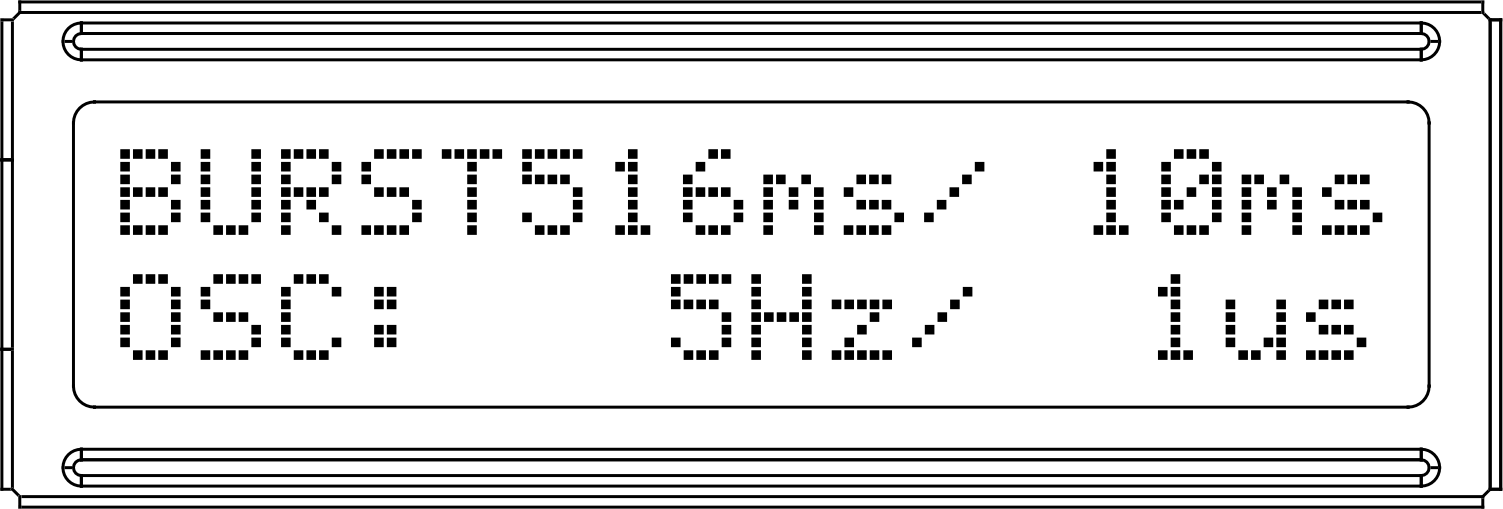
\includegraphics[width=100mm]{image/Arduino_Interrupter_v1_LCD_BURST.png}
\end{center}
\vspace*{5mm}

\subsection{操作方法}

\vspace*{5mm}
\begin{center}

\includegraphics[width=100mm]{image/Arduino_Interrupter_v1_Design_Burst.png}
\end{center}
\vspace*{5mm}

基本的にVR1・VR2・VR3・VR4を操作することにより周波数とON時間、バーストモードのOFF時間とON時間を設定します。

\vspace*{5mm}

\begin{table}[htbp]
\begin{center}
\begin{tabular}{ | c | c | }
\hline
\textbf{VR1} & 周波数変更(5Hz - 1018Hz @ 1Hz Step) \\\hline
\textbf{VR2} & ON時間変更(1us - 254us @ 1us Step) \\\hline
\textbf{VR3} & バーストOFF時間(516ms - 10ms @ 1ms Step) \\\hline
\textbf{VR4} & バーストON時間(10ms - 516ms @ 1ms Step ) \\\hline
\textbf{PUSH1} & 割当無し \\\hline
\textbf{PUSH2} & 割当無し \\\hline
\end{tabular}
\end{center}
\end{table}



\clearpage

\section{MIDI モード}

MIDIコネクタまたはUSB-MIDI経由で受信したMIDIの音程を出力するモードです。

\subsection{画面表示}

画面1行目にOUT1とOUT2が受信するMIDIチャンネルが表示されます。 \\
画面2行目にはOUT1 / 2 それぞれの受信したノートナンバーと設定されたON時間が表示されます。 \\
MIDIチャンネルの設定方法については後述します。

\vspace*{5mm}
\begin{center}
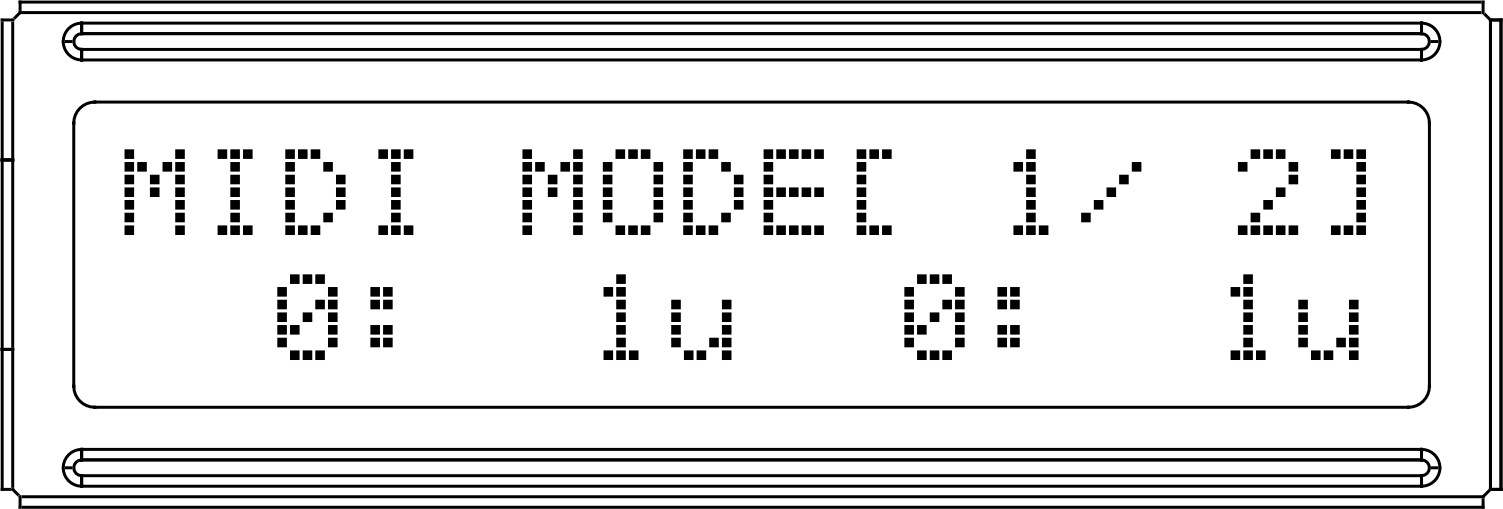
\includegraphics[width=100mm]{image/Arduino_Interrupter_v1_LCD_MIDI.png}
\end{center}
\vspace*{5mm}

\subsection{操作方法}

\vspace*{5mm}
\begin{center}

\includegraphics[width=100mm]{image/Arduino_Interrupter_v1_Design_MIDI.png}
\end{center}
\vspace*{5mm}

基本的にVR1とVR2を操作することによりON時間を設定します。

\vspace*{5mm}

\begin{table}[htbp]
\begin{center}
\begin{tabular}{ | c | c | }
\hline
\textbf{VR1} & OUT1 - ON時間変更(1us - 254us @ 1us Step) \\\hline
\textbf{VR2} & OUT2 - ON時間変更(1us - 254us @ 1us Step) \\\hline
\textbf{VR3} & 割当無し \\\hline
\textbf{VR4} & 割当無し \\\hline
\textbf{PUSH1} & 割当無し \\\hline
\textbf{PUSH2} & 割当無し \\\hline
\end{tabular}
\end{center}
\end{table}



\clearpage

\section{MIDI FIXED モード}

MIDI使用時にON時間が固定の場合、音程によって音圧が異なって聞こえるため、ON時間に補正をかけるモードです。

\subsection{画面表示}

画面1行目にOUT1とOUT2が受信するMIDIチャンネルと実際に出力されたON時間が表示されます。 \\
画面2行目にはOUT1 / 2 それぞれの受信したノートナンバーと設定されたON時間が表示されます。 \\
MIDIチャンネルの設定方法については後述します。

\vspace*{5mm}
\begin{center}
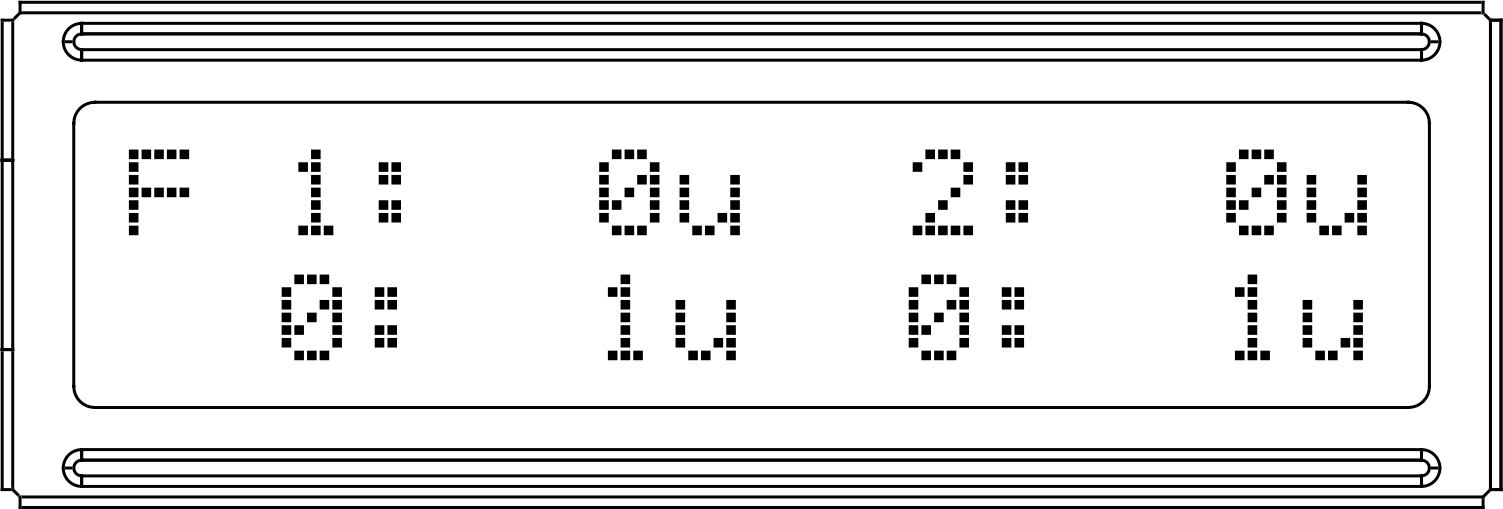
\includegraphics[width=100mm]{image/Arduino_Interrupter_v1_LCD_MIDI_FIX.png}
\end{center}
\vspace*{5mm}

\subsection{操作方法}

\vspace*{5mm}
\begin{center}

\includegraphics[width=100mm]{image/Arduino_Interrupter_v1_Design_MIDI_FIX.png}
\end{center}
\vspace*{5mm}

基本的にVR1とVR2を操作することにより最大ON時間を設定します。

\vspace*{5mm}

\begin{table}[htbp]
\begin{center}
\begin{tabular}{ | c | c | }
\hline
\textbf{VR1} & OUT1 - 最大ON時間変更(1us - 254us Max @ 1us Step) \\\hline
\textbf{VR2} & OUT2 - 最大ON時間変更(1us - 254us Max @ 1us Step) \\\hline
\textbf{VR3} & 割当無し \\\hline
\textbf{VR4} & 割当無し \\\hline
\textbf{PUSH1} & 割当無し \\\hline
\textbf{PUSH2} & 割当無し \\\hline
\end{tabular}
\end{center}
\end{table}



\clearpage

\section{設定変更(設定モード1)}

\subsection{設定モード1}

PUSH1を押したままインタラプター本体の電源をONにすることで設定モード1に入ります。 \\
拡張モードの使用(4-MODE / 2-MODE / 1-MODE)と出力確認用ビープスピーカーの使用が設定可能です。

\vspace*{10mm}
\begin{center}

\includegraphics[width=100mm]{image/Arduino_Interrupter_v1_LCD_SET_1.png}
\end{center}
\vspace*{10mm}

VR1を操作することにより拡張モードの使用(4-MODE / 2-MODE / 1-MODE)を切り替えます。 \\
VR2を操作することにより出力確認用ビープスピーカーの使用を切り替えます。

\vspace*{10mm}
\begin{center}
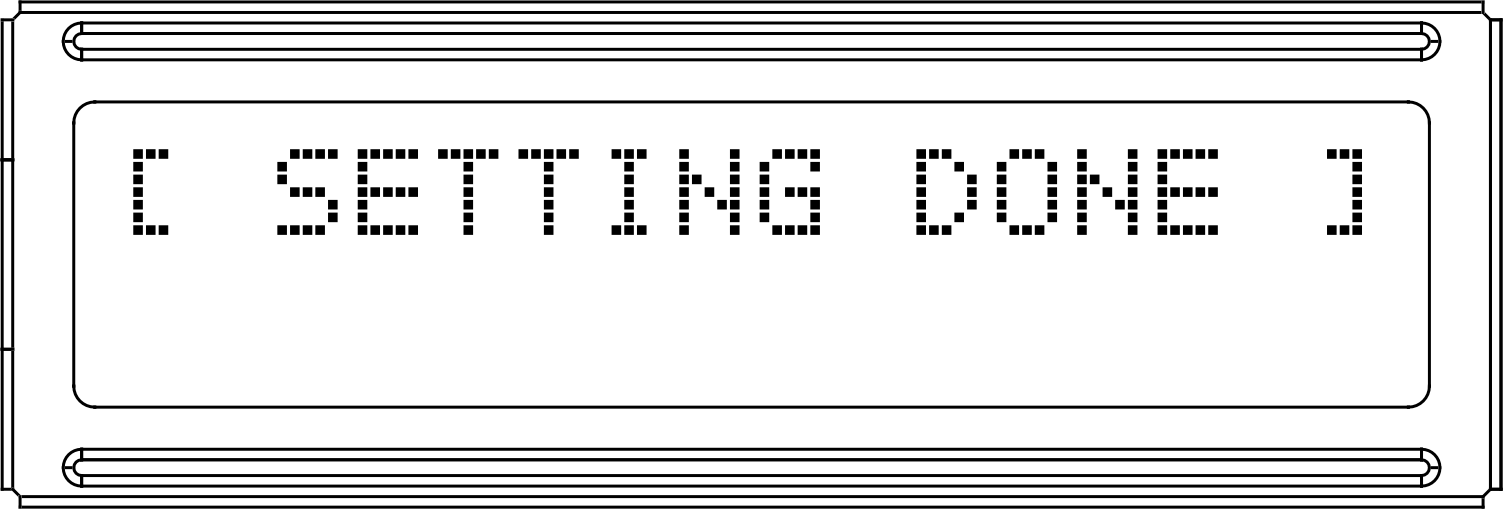
\includegraphics[width=100mm]{image/Arduino_Interrupter_v1_LCD_SET_DONE.png}
\end{center}
\vspace*{10mm}

PUSH2を押すことで設定が保存されます。 \\
PUSH2を押さずに電源をOFFにすることで設定を破棄できます。



\clearpage

\section{設定変更(設定モード2)}

PUSH2を押したままインタラプター本体の電源をONにすることで設定モード2に入ります。 \\
MIDIモード使用時の受信チャンネルについて設定可能です。

\vspace*{10mm}
\begin{center}
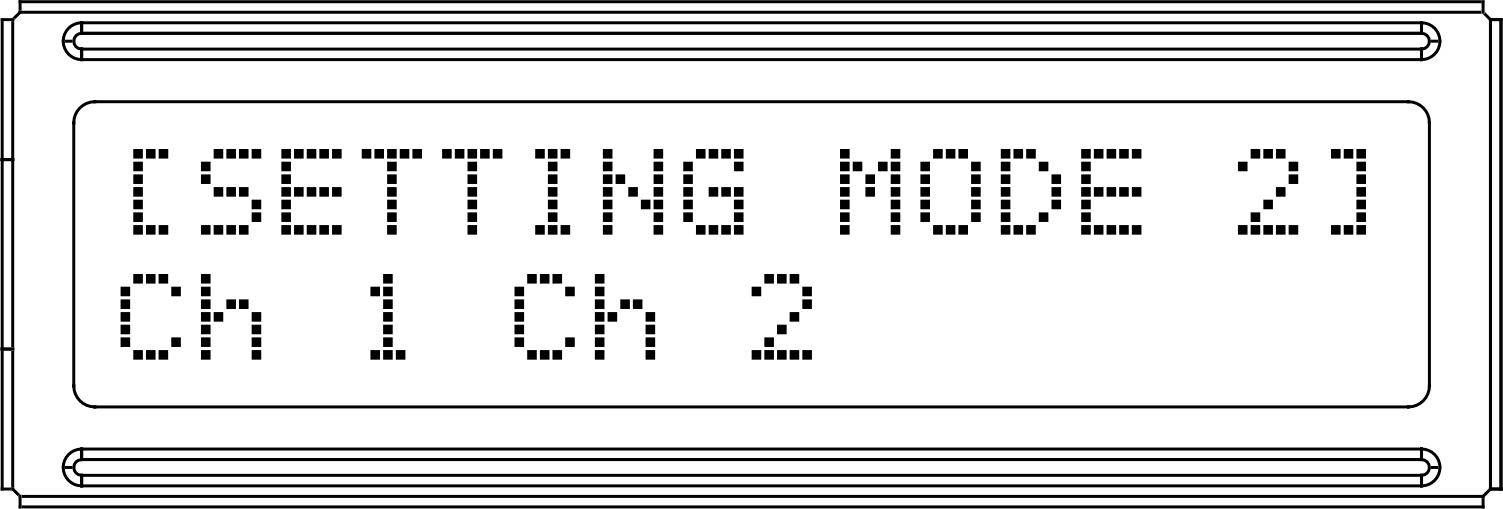
\includegraphics[width=100mm]{image/Arduino_Interrupter_v1_LCD_SET_2.png}
\end{center}
\vspace*{10mm}

VR1を操作することによりOUT1の受信チャンネルを設定します。 \\
VR2を操作することによりOUT2の受信チャンネルを設定します。 

\vspace*{10mm}
\begin{center}
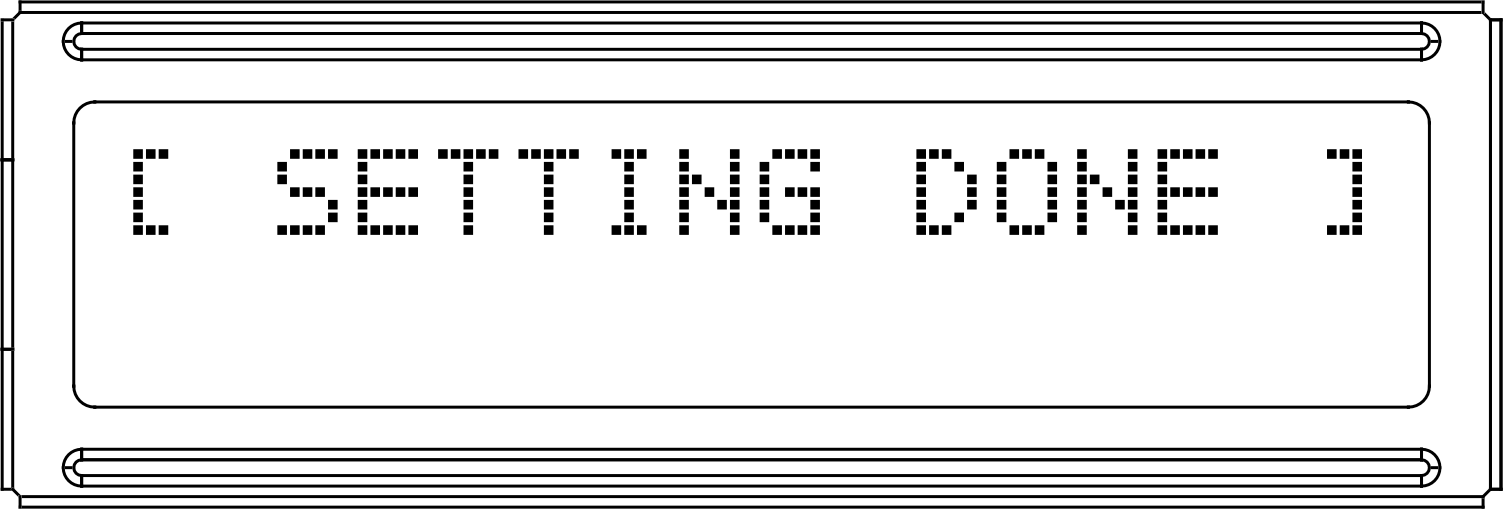
\includegraphics[width=100mm]{image/Arduino_Interrupter_v1_LCD_SET_DONE.png}
\end{center}
\vspace*{10mm}


PUSH1を押すことで設定が保存されます。 \\
PUSH1を押さずに電源をOFFにすることで設定を破棄できます。



\clearpage


\section{各種仕様}


\subsection{生成可能な波形}

出力信号は5Vの矩形波となります。

\begin{table}[htbp]
\begin{center}
\begin{tabular}{ | c | c | c | c | }
\hline
\textbf{操作モード} & \textbf{出力周波数} & \textbf{出力ON時間} & \textbf{備考} \\\hline
インタラプターモード & 5Hz - 1018Hz @ 1Hz Step & 1us - 254us @ 1us Step & 常時出力 \\\hline
ワンショットモード & 任意タイミング & 1us - 507us @ 1us Step & スイッチトリガー \\\hline
ハイパワーモード & 5Hz - 36Hz @ 1Hz Step & 0us - 12600us @ 100us Step & 常時出力 \\\hline
ハイパワーワンショットモード & 任意タイミング & 100us - 12700us @ 100us Step & スイッチトリガー \\\hline
バーストモード* & 5Hz - 1018Hz @ 1Hz Step & 1us - 254us @ 1us Step & 常時出力 \\\hline
MIDI モード & ノートナンバー & 1us - 254us @ 1us Step & ノートONトリガー \\\hline
MIDI FIXED モード & ノートナンバー & 1us - 254us Max @ 1us Step & ノートONトリガー \\\hline
\end{tabular}
\end{center}
\end{table}

*バーストモードの場合、
OFF時間 516ms - 10ms @ 1ms Step / 
ON時間 10ms - 516ms @ 1ms Step 
で変調できます。


\subsection{要求するハードウェア}
このファームウェアプログラムは以下のボードで動作します。専用ボードまたはArduino Microを推奨します。

\begin{table}[htbp]
\begin{center}
\begin{tabular}{ | c | c | c | c | }
\hline
\textbf{ボード名} & \textbf{搭載マイコン} & \textbf{出力数} & \textbf{USB-MIDI対応} \\\hline
\textbf{HTLAB.NET Arduino DRSSTC Interrupter Ver 1.0} & ATmega32u4 & 2 & 対応 \\\hline
\textbf{Arduino Micro} & ATmega32u4 & 2 & 対応 \\\hline
\textbf{Arduino Leonardo} & ATmega32u4 & 2 & 対応 \\\hline
\end{tabular}
\end{center}
\end{table}

\subsection{要求するソフトウェア}
Arduino IDE 1.8.1 以降 
(https://www.arduino.cc/en/Main/Software)

Arduino MIDI Library 4.3.1 以降 
(https://playground.arduino.cc/Main/MIDILibrary)

MIDIUSB library 1.0.3 以降 
(https://www.arduino.cc/en/Reference/MIDIUSB)


\subsection{ファームウェアファイル構成}

\begin{table}[htbp]
\begin{center}
\begin{tabular}{ | c | c | }
\hline
\textbf{ファイル名} & \textbf{ファイル内容} \\\hline
\textbf{HTLAB.NET\_Arduino\_DRSSTC\_Interrupter.ino} & Arduinoメインプログラム \\\hline
\textbf{lib\_input.cpp} & ピン入力に関するプログラム \\\hline
\textbf{lib\_input.h} & ピン入力に関するヘッダファイル \\\hline
\textbf{lib\_midi.h} & MIDI関係定義ヘッダファイル \\\hline
\textbf{lib\_osc.cpp} & 発振器操作に関するプログラム \\\hline
\textbf{lib\_osc.h} & 発振器操作に関するヘッダファイル \\\hline
\textbf{lib\_output.cpp} & ピン出力に関するプログラム \\\hline
\textbf{lib\_output.h} & ピン出力に関するヘッダファイル \\\hline
\textbf{settings.h} & 設定定義ヘッダファイル \\\hline
\end{tabular}
\end{center}
\end{table}







\clearpage

\section{プログラムの設定方法}
ファームウェアプログラムの設定を変更する場合「settings.h」ファイルを編集します。 \\

\begin{table}[htbp]
\begin{center}
\begin{tabular}{ | c | c | c |}
\hline
\textbf{定数名} & \textbf{初期値} & \textbf{概要} \\\hline
USE\_LCD & true & キャラクターLCDを使用する \\\hline
USE\_VR1 & true & VR1を使用する \\\hline
USE\_VR2 & true & VR2を使用する \\\hline
USE\_VR3 & true & VR3を使用する \\\hline
USE\_VR4 & true & VR4を使用する \\\hline
INVERT\_VR1 & false & VR1の動作を反転させる \\\hline
INVERT\_VR2 & false & VR2の動作を反転させる \\\hline
INVERT\_VR3 & false & VR3の動作を反転させる \\\hline
INVERT\_VR4 & false & VR4の動作を反転させる \\\hline
DEFAULT\_VR1 & 0 & VR1の初期値設定(VR1未使用時) \\\hline
DEFAULT\_VR2 & 0 & VR2の初期値設定(VR2未使用時) \\\hline
DEFAULT\_VR3 & 0 & VR3の初期値設定(VR3未使用時) \\\hline
DEFAULT\_VR4 & 0 & VR4の初期値設定(VR4未使用時) \\\hline
USE\_SW1 & true & SW1を使用する \\\hline
USE\_SW2 & true & SW2を使用する \\\hline
INVERT\_SW1 & false & SW1の動作を反転させる \\\hline
INVERT\_SW2 & false & SW2の動作を反転させる \\\hline
DEFAULT\_SW1 & false & SW1の初期値設定(SW1未使用時) \\\hline
DEFAULT\_SW2 & false & SW2の初期値設定(SW2未使用時) \\\hline
USE\_PUSH1 & true & PUSH1を使用する \\\hline
USE\_PUSH2 & true & PUSH2を使用する \\\hline
INVERT\_PUSH1 & false & PUSH1の動作を反転させる \\\hline
INVERT\_PUSH2 & false & PUSH2の動作を反転させる \\\hline
USE\_SETTING\_MODE & true & 起動時に設定モードを使用する \\\hline
DEFAULT\_MODE\_SELECTOR & 0 & 初回起動時に使用する拡張モード(4-Mode) \\\hline
DEFAULT\_BEEP\_ACTIVE & 1 & 初回起動時のビープスピーカー使用設定 \\\hline
DEFAULT\_MIDI\_CH1 & 1 & 初回起動時のMIDIチャンネル設定(OUT1) \\\hline
DEFAULT\_MIDI\_CH2 & 2 & 初回起動時のMIDIチャンネル設定(OUT2) \\\hline
MIDI\_MAX\_NOTE\_NUM\_CH1 & 84 & 発音可能の最大MIDIノートナンバー(OUT1) \\\hline
MIDI\_MAX\_NOTE\_NUM\_CH2 & 84 & 発音可能の最大MIDIノートナンバー(OUT2) \\\hline
USE\_MIDI & true & MIDIポートを使用する \\\hline
USE\_MIDIUSB & true & USB接続の際にUSB-MIDIとして使用する \\\hline
\end{tabular}
\end{center}
\end{table}



\clearpage

\section{プログラムの書き込み方法}

Arduino IDEにて「HTLAB.NET\_Arduino\_DRSSTC\_Interrupter.ino」を開きます。 \\
設定内容に応じて、以下のライブラリが必要になります。 \\

Arduino MIDI Library 4.3.1 以降 
(https://playground.arduino.cc/Main/MIDILibrary)

MIDIUSB library 1.0.3 以降 
(https://www.arduino.cc/en/Reference/MIDIUSB)
\\

ボードを指定して書き込めば動作します。\\

HTLAB.NET Arduino DRSSTC Interrupter Ver 1.0を使用する場合はブートローダーの書き込みが必要です。 \\

例としてWindows上のArduino IDEからAVRISP mkIIを使用してブートローダーを書き込む場合は、libusb-win32がインストールされている必要があります。 
フィルタードライバをインストールの上、ブートローダー書き込みを実行してください。 \\


\section{Arduino Microを使用した場合の配線方法}

Arduino Microを使用してインタラプターを製作することが可能です。 \\
キャラクターLCDを使用する場合、コントラスト調整用の半固定抵抗を忘れないようにしてください。 \\
また、LCDのR/Wピンは必ずGNDに落とし、DB0 - 3もノイズ対策のためにGNDに落とすことを推奨します。

\begin{table}[htbp]
\begin{center}
\begin{tabular}{ | c | c | c |}
\hline
\textbf{ピン番号} & \textbf{接続先} & \textbf{概要} \\\hline
D0(RX)  & MIDI IN & フォトカプラでMIDI信号を受信してください(PC900V/6N138/TLP2361 等) \\\hline
D1(TX)  & (MIDI OUT) & 現段階では未使用です \\\hline
D2  & PUSH1 & プッシュスイッチに接続し、その先をGNDに落としてください(内部Pull-Up済) \\\hline
D3  & PUSH2 & プッシュスイッチに接続し、その先をGNDに落としてください(内部Pull-Up済) \\\hline
D4  & LCD (RS) & 16文字2行キャラクターLCD「Register Select」ピンに接続してください \\\hline
D5  & LCD (ENA) & 16文字2行キャラクターLCD「Enable Signal」ピンに接続してください \\\hline
D6  & LCD (DB4) & 16文字2行キャラクターLCD「Data Bit 4」ピンに接続してください \\\hline
D7  & LCD (DB5) & 16文字2行キャラクターLCD「Data Bit 5」ピンに接続してください \\\hline
D8  & LCD (DB6) & 16文字2行キャラクターLCD「Data Bit 6」ピンに接続してください \\\hline
D9  & LCD (DB7) & 16文字2行キャラクターLCD「Data Bit 7」ピンに接続してください \\\hline
D10 & OUT1 & 信号の出力です。フォトカプラ等で必ず絶縁して使用してください \\\hline
D11 & OUT2 & 信号の出力です。フォトカプラ等で必ず絶縁して使用してください \\\hline
D12 & LCD BL & LCDバックライト制御信号線。常時点灯や常時不点灯の場合は未使用 \\\hline
D13 & PIEZO & 圧電スピーカーに接続し、その先をGNDに落としてください \\\hline
A0  & VR1 & 5V - GND間に接続したボリュームの中点を接続してください。0V - 5Vの入力です \\\hline
A1  & VR2 & 5V - GND間に接続したボリュームの中点を接続してください。0V - 5Vの入力です \\\hline
A2  & VR3 & 5V - GND間に接続したボリュームの中点を接続してください。0V - 5Vの入力です \\\hline
A3  & VR4 & 5V - GND間に接続したボリュームの中点を接続してください。0V - 5Vの入力です \\\hline
A4  & SW1 (MIDI) & トグルスイッチに接続し、その先をGNDに落としてください(内部Pull-Up済) \\\hline
A5  & SW2 (MODE) & トグルスイッチに接続し、その先をGNDに落としてください(内部Pull-Up済) \\\hline
\end{tabular}
\end{center}
\end{table}



\clearpage
\newgeometry{top=1truecm, bottom=1truecm, left=1truecm, right=1truecm}

\begin{center}
\huge{MIDIインプリメンテーションチャート}
\end{center}

\begin{flushright}
\small{HTLAB.NET Arduino DRSSTC Interrupter \hwVer  (FW:\fwVer)}
\end{flushright}

\begin{table}[htbp]
\begin{center}
\begin{tabular}{ | p{2cm} p{2cm} | p{4cm} | p{4cm} | p{4cm} | }
\hline
\multicolumn{2}{|c|}{\textbf{\large ファンクション}} & 
\multicolumn{1}{c|}{\textbf{\large 送信}} & 
\multicolumn{1}{c|}{\textbf{\large 受信}} & 
\multicolumn{1}{c|}{\textbf{\large 備考}} \\\hline


\textbf{ベーシック} & \multicolumn{1}{r|}{電源ON時} & \midFalse & 1-16 & チャンネル設定可能 \\
\textbf{チャンネル} & \multicolumn{1}{r|}{設定可能} & \midFalse & \midFalse & \\\hline

 & \multicolumn{1}{r|}{電源ON時} & \midFalse & モード3 & \\
\textbf{モード} & \multicolumn{1}{r|}{メッセージ} & \midFalse & \midFalse & \\
 & \multicolumn{1}{r|}{代用} & \midFalse & \midFalse & \\\hline

\textbf{ノート} & & \midFalse & 0-127 & 制限可能(既定値:0-84) \\
\textbf{ナンバー} & \multicolumn{1}{r|}{:音域} & \midFalse & 0-127 & タイマ8分周時下限24 \\\hline

\multirow{2}{*}{\textbf{ベロシティ}} & \multicolumn{1}{r|}{ノート・オン} & \midFalse & \midFalse & ボリュームにて強制設定 \\
 & \multicolumn{1}{r|}{ノート・オフ} & \midFalse & \midFalse &  \\\hline

\textbf{アフター} & \multicolumn{1}{r|}{キー別} & \midFalse & \midFalse & \\
\textbf{タッチ} & \multicolumn{1}{r|}{チャンネル別} & \midFalse & \midFalse & \\\hline

\textbf{ピッチベンド} & & \midFalse & \midFalse & \\\hline




\end{tabular}
\end{center}
\end{table}
\thispagestyle{empty}
\restoregeometry




\end{document}


